Auf Basis der dimensionierten Haut und des Holms soll ein CAD-Modell des Flügels erstellt werden. Zur Konstruktion wird das CAD-Programm Solid Edge in der Studentenversion verwendet. Als Grundlage dient eine gegebene unvollständig bemaßte technische Zeichnung der Profilkontur, aus der exakt entnommen werden kann, dass das Profil ohne die Hochauftriebselemente oder Querruder von einem Rechteck der Kantenlängen $ 172mm $, dies entspricht der Profiltiefe, und $ 37,5mm $ gerade umschlossen wird. Aus den bekannten Längenangaben kann der Maßstab der gedruckten Zeichnung bezüglich des Modellmaßstabs zu $ 1:1,039 $ berechnet werden. Markante Punkte entlang der Kontur können in der Zeichnung vermessen werden und mithilfe des Maßstabs auf Punkte im CAD-Modell umgerechnet werden. Im CAD-Programm werden Tangentenbögen von Punkt zu Punkt gelegt, um die Kontur hinreichend glatt anzunähern. Die verwendeten Punkte werden durch die im Anhang befindliche technische Zeichnung der Profilkontur illustriert.\\

\subsubsection{Konstruktion der Gurte}
\label{GurtKonstrukt}
\noindent In den Bereichen oberhalb und unterhalb des Holms soll die Haut nicht in Sandwich-Bauweise ausgeführt sein. Für die Auslegung des Holms wurde davon ausgegangen, dass eine Dicke des Verbundmaterials der Haut von $ 0,75mm $ ausreichend ist, die nach Gleichung ~\ref{gurtlagen} 9 Lagen des Interglas 90070 Gewebes entspricht. Die genauere Auslegung der Haut hat gezeigt, dass nur zwei Lagen des Gewebes notwendig sind. Der entstehende Freiraum $t_{frei}= 0,75mm-2\cdot 0,078mm=0,594mm $ zwischen der Haut und den weiter innen liegenden Gurten kann bei der Fertigung mit Harz aufgefüllt werden.\\
\noindent Der zu Beginn des Abschnitts ~\ref{GurtDim} dimensionierte Holm mit rechteckigen Gurtquerschnitten, $ b=28mm $ und $ h_{a}=36mm $, wird nun so auf die Kontur des Profils gelegt, dass die Überdeckung der Gurte mit der umgebenden Haut möglichst gering ausfällt. Dann wird die Höhe $ h_{a} $ an den örtlichen inneren Abstand der oberen und unteren Haut auf $\tilde{h_{a}}=35,8mm $ angepasst. Der rechteckige Querschnitt der Gurte wird mithilfe eines Offsets von $ {h}=1,941mm $ der Hautkrümmung angepasst. Diese Anpassungsmaßnahmen senken das Flächenträgheitsmoment leicht. Das resultierende Flächenträgheitsmoment $ \tilde{I_{x}} $ lässt sich aufgrund der komplexen Querschnittsgeometrie der Gurte nur mit dem CAD-Programm exakt bestimmen. 
\begin{figure}[h]
	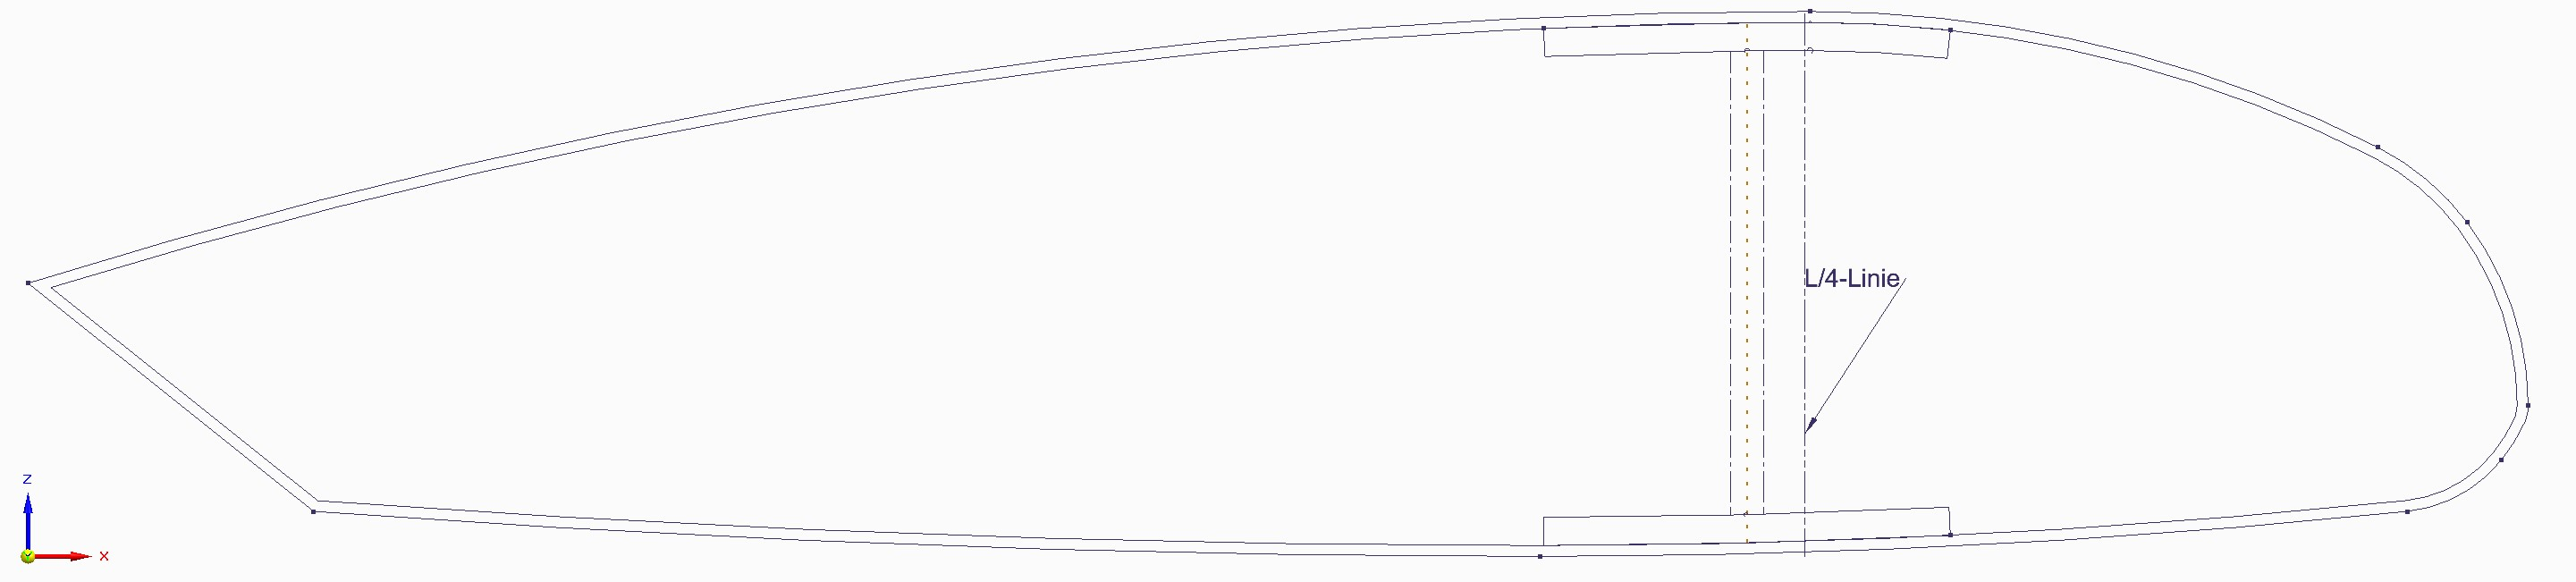
\includegraphics[width=1.0\textwidth]{Bilder/Kontur.jpg}
	\caption{Haut und Gurte nach dem ersten Schritt der Konstruktion}
	\label{fig: Kontur}
\end{figure} 
Der Vergleich mit dem erforderlichen Flächenträgheitsmoment zeigt, dass die angepasste Geometrie der Gurte die Steifigkeitsbedingung (vgl. Beziehung ~\ref{IVergleich}) erfüllt. Die Haut konstanter Dicke und die Gurte im ersten Schritt der Konstruktion werden durch Abbildung ~\ref{fig: Kontur} veranschaulicht. Zusätzlich zeigt die Abbildung die ungefähre Lage der L/4-Linie. Diese wurde mithilfe einer vorhandenen Hilfsansicht der Tragfläche inklusive der Hinterkantenklappen und des Vorflügels, beide im eingefahrenen Zustand, ermittelt. In der Hilfsansicht wird die abgebildete Länge des mittleren auszulegenden Teils der Tragfläche gemessen. Der Maßstab der ausgedruckten Hilfsansicht bezüglich des Modellmaßstabes wird zu 1:2,529 berechnet. Diese Kenntnis ermöglicht die Berechnung des Abstandes der L/4-Linie zur Vorderkante der Haupttragfläche, der $ 42,4mm $ beträgt und besonders für die Berechnung der Torsion ausschlaggebend ist.\\

\subsubsection{Konstruktion des Stegs}
\noindent Im nächsten Schritt werden die beiden Stegseiten und der in der Mitte liegende Schaum konstruiert. Im CAD-Programm erfolgt dies mithilfe von nur einer Skizze, die der Extrusion der Einzelteile zugrunde liegt.So kann sichergestellt werden, dass in jeder Komponente der Bezug auf die angrenzenden Gurte und die unterschiedlichen Krümmungsradien der Seitenkanten gewahrt bleibt. Die Konstruktionen des Steges und des Schaumes erfordern auch die Berücksichtigung der verschieden belegten Unterteilungen des Steges. Während der innere Teil des Stegs, am inneren Holmstummel-Ende beginnend und $ 23mm $ in $y$-Richtung über die Aufnahme der Querkraftbolzen an Punkt C hinaus gehend, gemäß der Dimensionierung mithilfe des Laminatrechners mit 24 Lagen aufgeteilt zu jeweils zwölf Lagen auf beiden Seiten des Schaums belegt wird, soll der gesamte äußere Teil mit nur insgesamt vier Lagen gleichmäßig verteilt belegt werden. Es bietet sich an, die vier Lagen des äußeren Bereichs über die gesamte Holmlänge zu erstrecken. Die 20 verstärkenden Lagen enden $ 23mm $ hinter Punkt C in einem sanften Übergang mit einer Länge von $ 30mm $. Der dünn belegte Teil wird durch einen $ 2mm $ breiten Schaumkern vor dem Beulen geschützt, der zum dick belegten Teil hin entsprechend schmaler wird. Das innere Holmstummel-Ende wird auf eine Länge von $ l_{0}=30mm $ im Abstand vom Mittelpunkt des Lagers A abgeschätzt. Abbildung ~\ref{fig: Steg} veranschaulicht den prinzipiellen Aufbau. Eine technische Zeichnung im Anhang illustriert die Konstruktion von Gurten und Steg. Sie gibt außerdem Aufschluss über die wichtigsten Maße und stellt die unterschiedlichen Wandstärken des Schaumkerns und des Faserverbundanteils im Steg für die verschiedene Bereiche im Querschnitt grafisch dar.

\begin{figure}[h]
	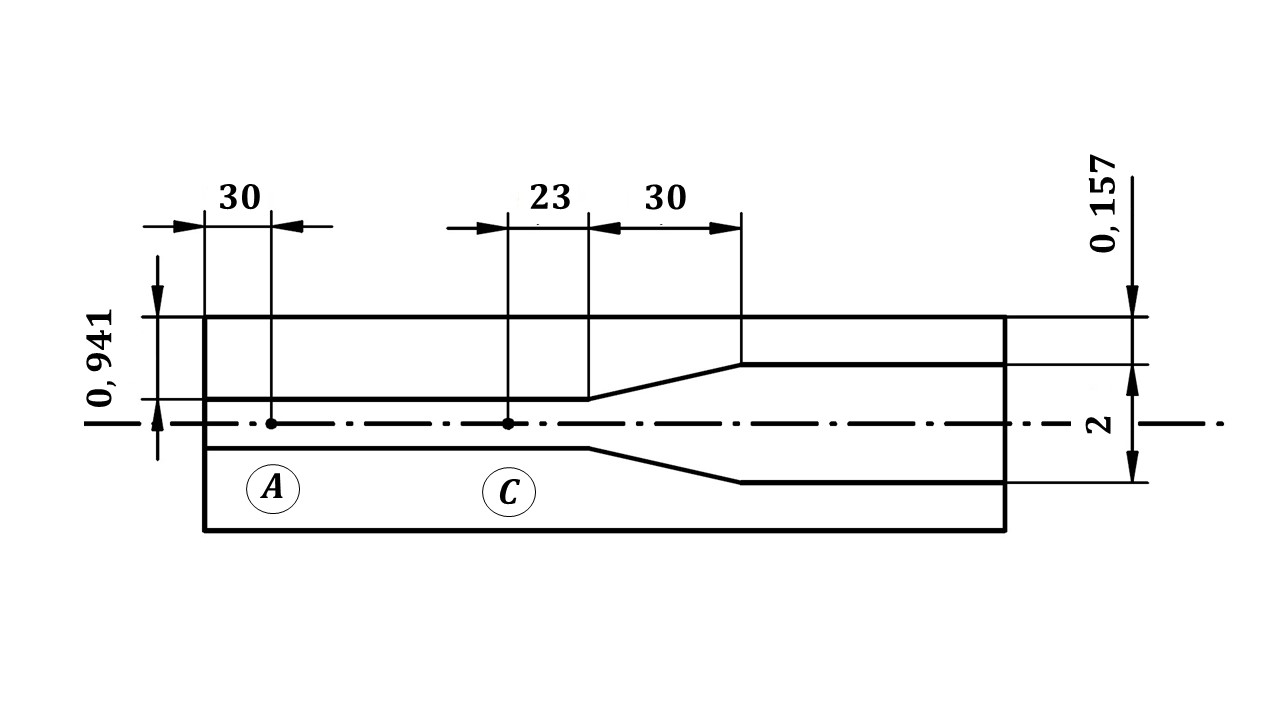
\includegraphics[width=1.0\textwidth]{Bilder/StegPrinzip.jpg}
	\caption{Prinzipskizze der Sandwichstruktur im Steg}
	\label{fig: Steg}
\end{figure}


\subsubsection{Konstruktion der Haut und der Rippen}
Um die Haut vor Beulerscheinungen zu schützen, soll ein Schaumkern zwischen die innere und äußere Hautschicht gelegt werden. Der Beulberechnung ist zu entnehmen, dass mit einem $ 3mm $ dicken Kern ausreichende Sicherheit gegen Beulen gegeben ist. Ein Schaumkern dieser Stärke ist darüber hinaus gut handhabbar und kann mithilfe eines heißen Drahtes einfach und kostengünstig aus einem Styrodurklotz ausgeschnitten werden. Um die Höhe $ h_{a} $ der Gurte möglichst nicht durch die Haut einzuschränken, soll der Schaumkern zu den Gurten hin über $ 5mm $ in einem sanften Übergang auslaufen, sodass nur das Laminat über dem oberen und unter dem unteren Gurt hergeführt werden muss. Abbildung ~\ref{fig: Hautuebergang} veranschaulicht die prinzipielle Gestaltung der Haut im Bereich des oberen Gurtes, der grau dargestellt ist. \\

\noindent Der Freiraum zwischen Gurten, den Steglagen und der inneren Hautlage kann nun für die Vorder- und Hinterseite des Steges umrandet werden. Die darauf basierende Skizze ist die Grundlage der Konstruktion der zweigeteilten Wurzel- und Endrippe. Die Rippen werden in ihrer Dimensionierung als gegeben angenommen, eine Auslegung erfolgt im Rahmen dieser Projektarbeit nicht. Ein Belastungstest der Tragfläche würde in der Realität durch eine an der Endrippe angreifende Last erfolgen. Damit die Last angeschlagen werden kann, müssen zwei Bohrungen in der Endrippe vorgesehen werden, deren Abstand durch das gegebene Bauteil Endscheibe bestimmt wird. Zur einfachen Montage der Prüfeinheit werden zwei Gewindehülsen konstruiert, die in die Bohrungen eingefügt werden.

\begin{figure}[h]
	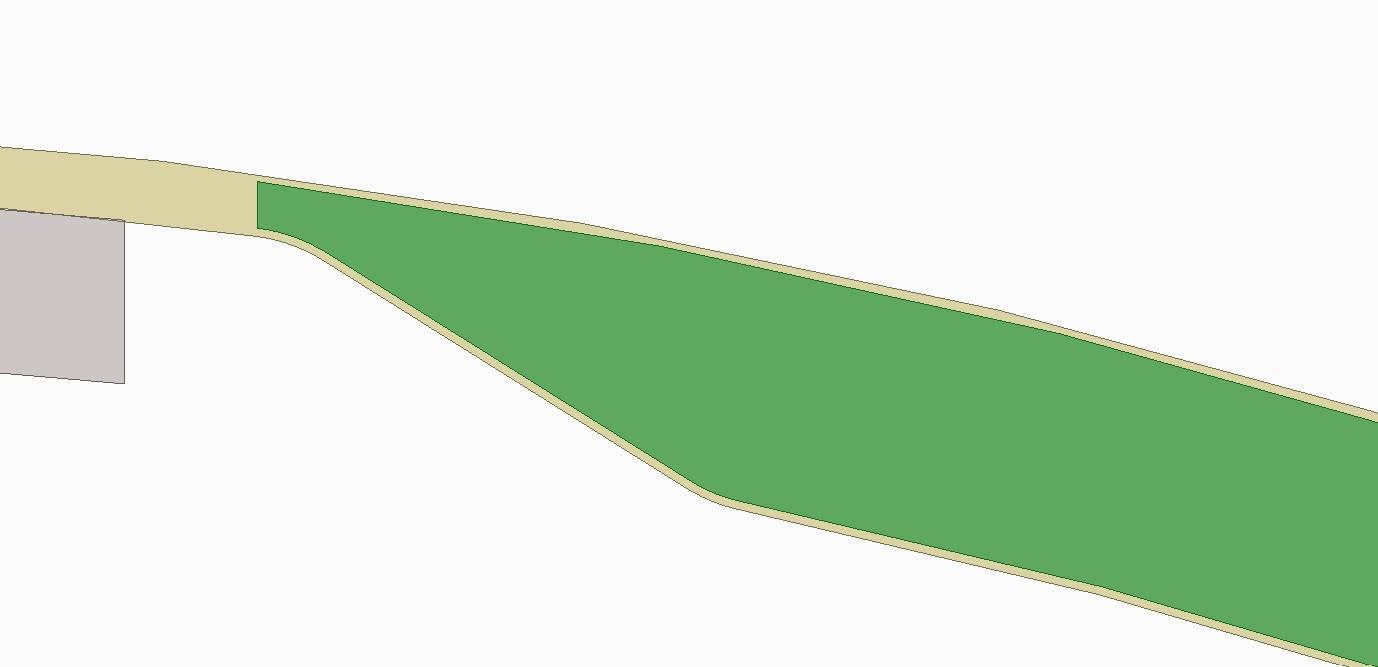
\includegraphics[width=1.0\textwidth]{Bilder/Hautuebergang.jpg}
	\caption{Hautsandwich am Übergang zum Gurt}
	\label{fig: Hautuebergang}
\end{figure}

\subsubsection{Konstruktion unterstützender Bauteile des Holms}
Die Kraftaufnahme der  als Fest- und Loslager modellierten Punkte A und B erfolgt durch zwei Hauptbolzen, die im Flugzeug die Tragflächen miteinander verbinden. In diesem Fall werden die Lagerkräfte von maximal $ 5085N $ an den Teststand übertragen. Damit bei der Krafteinleitung in den Holm Spannungsspitzen vermieden werden, soll die Auflagefläche der Bolzen vergrößert werden. Dies geschieht, indem eine Holzkonstruktion für Vorder- und Rückseite des Holms erstellt wird, die der Kontur der Gurte angepasst ist und Bohrungen für die Bolzen enthält. Diese Klötze werden auf ihrer jeweiligen Stegseite mit den Gurten und dem Steg verklebt. Da der Abstand der Bohrungen mit $ 76mm $ gering ist, wird ein längerer Holzklotz für beide Bohrungen konstruiert. Aussparungen an den Seiten und zwischen den Bohrungen sollen das Gewicht der Klötze reduzieren. Zum Schutz der Hauptbolzen werden zwei Messinghülsen konstruiert und in die Bohrungen eingefügt. So kann verhindert werden, dass die gefetteten Bolzen bei Montage und Demontage Späne aus dem Steg lösen oder sich verkanten. Die Messinghülsen weisen eine Wandstärke von $ 0,5mm $ und einen Innendurchmesser von $ 8mm $ auf. In der Fertigung kann auf kostengünstige Messingrohre zurückgegriffen werden. Die Konstruktion wird durch Abbildung ~\ref{fig: Klotz} veranschaulicht. Eine technische Zeichnung des vorderen Holzklotzes mit Angaben zu den Hauptabmessungen befindet sich im Anhang.
\begin{figure}[h]
	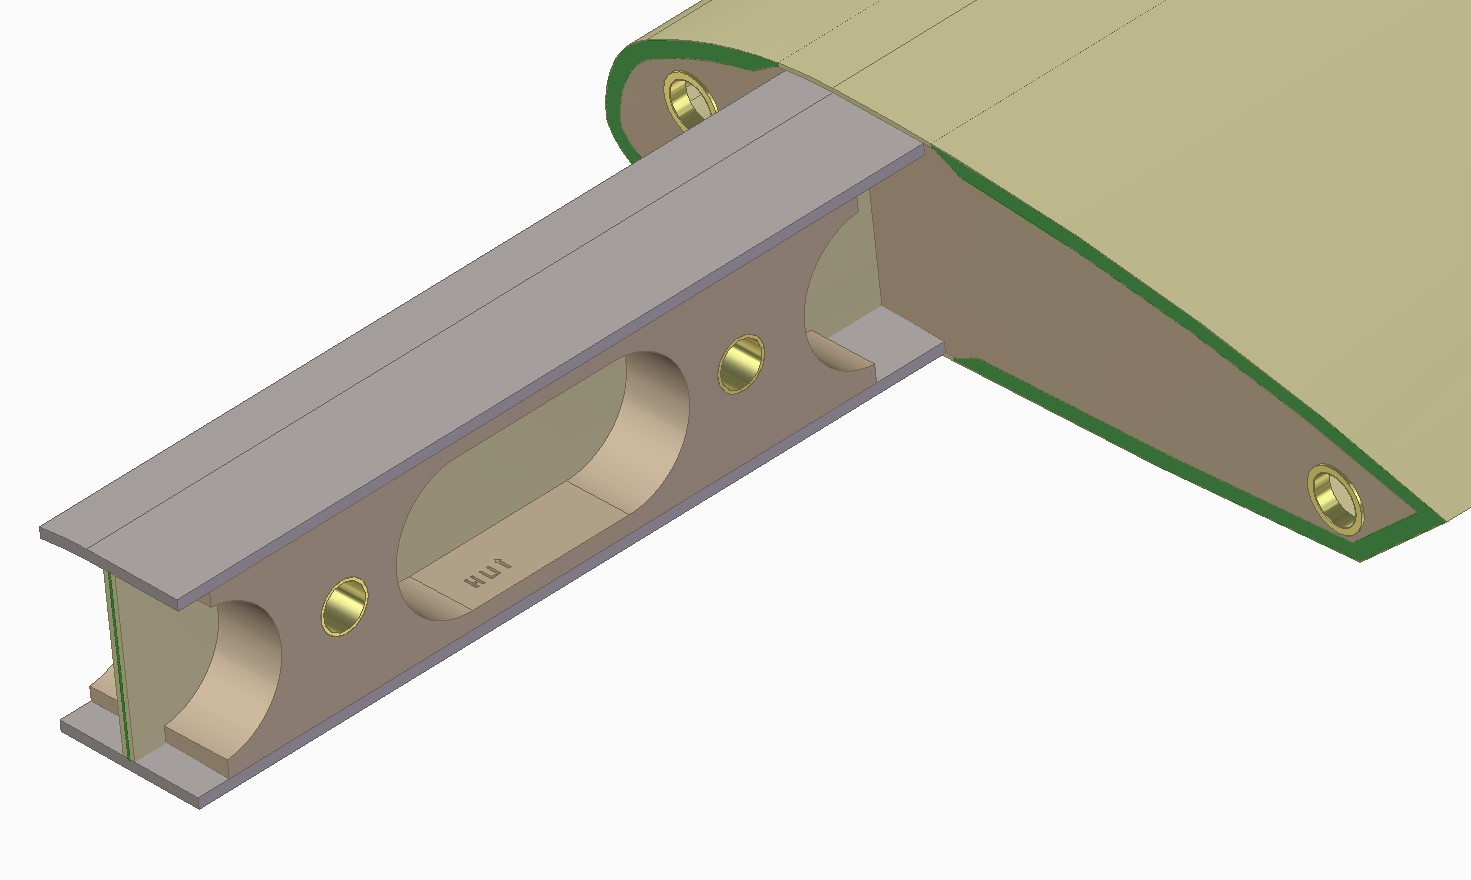
\includegraphics[width=1.0\textwidth]{Bilder/Klotz.jpg}
	\caption{Holzklötze und Hülsen}
	\label{fig: Klotz}
\end{figure}

\subsubsection{Querkraftbolzen und Montage auf dem Teststand}
Die Prüfung, ob die gesamte Auslegung der Tragfläche den Bestimmungen der Aufgabenstellung gerecht wird, erfolgt anhand einer FEM-Berechnung, anstelle der tatsächlichen Fertigung des Flügels und des Bruchtests. Dennoch kann mithilfe gegebener Zeichnungen der Teststandelemente geprüft werden, ob die konstruierte Tragfläche in der Realität auf dem Teststand montierbar wäre. Der Abstand der Hauptbolzen zueinander wurde bereits in der frühen Modellierung des Holms als Biegebalken berücksichtigt. Für die Positionierung der Bohrungen und Hülsen der Querkraftbolzen wird der Abstand zwischen den Langlöchern und der Aussparung für den Holm in der Montageplatte gemessen. An der gegenüberliegenden Wurzelrippe können so die Bohrungen festgelegt werden. Bei Verwendung der Maße aus der gegebenen technischen Zeichnung der Montageplatte, fällt auf, dass das Langloch zur Aufnahme des in Flugrichtung hinteren Querkraftbolzens für diese Konstruktion ungeeignet ist. Es liegt außerhalb des Bereichs der Wurzelrippe. Dies wird auf die Anordnung des Holms in der Tragfläche zurückgeführt, die die Position der Flügelkontur bezüglich der Montageplatte festlegt. Sie kann nachträglich nicht ohne größere Änderungen des Holmquerschnitts und eine damit verbundene Neuauslegung verändert werden. Abbildung \ref{fig: SeiteRichtig} des Anhangs veranschaulicht die ursprüngliche Lage des hinteren Langlochs. Um eine grundsätzlich neue Dimensionierung aller Komponenten zu vermeiden, wurde die Position des Langlochs angepasst. Da die Querkraftbolzen einen großen Abstand zueinander aufweisen (vgl. Abb. \ref{fig: Klotz}), müssen zur Aufnahme der Torsionsmomente nur kleine zusätzliche Kräfte aufgenommen werden. Die Radien der Langlöcher in der Montageplatte begrenzen den Durchmesser der Querkraftbolzen auf maximal $ 8,5mm $. Gemäß \ref{Bolzenberechnung} ist bereits ein Durchmesser von $ 8mm $ ausreichend. Auch für die Querkraftbolzen werden Hülsen konstruiert, die die Wurzelrippe schützen und die Montage erleichtern. Sie sind in Abbildung \ref{fig: Klotz} ebenfalls dargestellt.\\

\noindent Alle Komponenten der Tragfläche und ihre Positionen sind im Anhang auf einer Explosionszeichnung ersichtlich. Eine Grafik des gesamten CAD-Modells und der Bauteile des Teststandes ist ebenfalls im Anhang enthalten (vgl. Abb. \ref{fig:AufbauGesamt}).Abbildung \ref{fig:MontagePlatte} zeigt die auf der Montageplatte positionierte Tragfläche unter Verwendung des angepassten Langlochs.
